\section{Data provided by REM observations}
\protect\label{section:tdataprovided}

\subsection{Data Available}

Consideration of the data available from the Red Dots project site is
hereinafter restricted to the targets of the project, the {\rdwarf} stars,
\prox, {\bstar} and \ross. The relevant data available is.

\begin{itemize}
 \item Images taken with visible light filters \textbf{g},
\textbf{i}, \textbf{r} and \textbf{z} taken almost daily. although not
necessarily of the REM {\rdwarf} targets, especially during April through to the
first part of July each year when the position of the Sun in the sky makes
observations impossible. All the images of the REM {\rdwarf} targets are taken
at a gain of 1 and the other targets with a gain of 4.4. 
\item Sky flat file images taken almost every day, usually as 3 images from the
sky, taken as the light fades. A set is taken with a gain of 4.4 and with a gain
of 1 each time, even if no observations are taken with that gain.
\item Bias file images taken each day
approximately 8 hours after the observations.
\item There are a very small number of dark file images (as for bias but with
an exposure of other than zero) taken in 2015, but these were from two years
before before the {\rdwarf} observations were commenced and are disregarded
herein.
\item Monthly master flat file images for each month constructed from some of
the daily flat files for the month in question.
\item Monthly master bias file images for each month, constructed from some of
the daily bias files for the month in question.
\item REMIR infrared images taken almost every day up to June 2019. These are
already reduced with the PREPROCESS software \citep{dipaola01}.
\item IDL routines used to prepare the master bias and flat files.
\end{itemize}

The flat and bias images are only available for the visible light filters \textbf{g},
\textbf{i}, \textbf{r} and \textbf{z} as the REMIR images have already been
processed. Except in a small handful of cases dating back to 2015, two years
before the {\rdwarf} observations started, these and the observation files all come as batches of four one for each filter, all
taken with the same exposure at the same time and in the case of observations,
looking at the same patch of sky.

The ROSS2 observations of the {\rdwarf} targets are all made with a gain of 1,
whilst all but one of the other targets observed in other projects were observed
with a gain of 4.4. Half of the daily flat and bias files are made with a gain
of 1 and the remainder with a gain of 4.4, even if no observations with a
particular gain are made. As this study is only considering the {\rdwarf}
targets, the only flat and bias files considered are those with a gain of 1.
The master flat and bias files are constructed from the daily flat and bias
files with a gain of 1.

The ROSS2 image files are stored with as 1024x1024 images, however the area of
the images is less than this as illustrated in Fig. \ref{fig:showusedccd}, the
upper and rightmost parts of the images are filled with zeros to make up to 1024
rows or columns. In all processing herein, the images are trimmed to the
appropriate size to avoid unnecessary computations with rows and columns of
zeros.

The REMIR infrared images, from the three filters \textbf{H}, \textbf{J} and
\textbf{K}. are divided approximately equally between 7 dither patterns. They
are 512x512 pixels in size and no flat or bias files are provided as
processing has already been done. Due to technical issues, they were
discontinued at the start of June 2019 and resumed in February 2021. A gain of 5
is applied to all the observations from the infrared images.

\subsection{Initial analysis of data}
\protect\label{section:initialanalysis}

The images are processed according to the formula:

\begin{center}
$ \frac{(mage - bias) \times mf}{flat - bias}$
\end{center}

In this $mf$ represents to mean value of the flat pixels. The master flat files
provided already have the bias subtracted. They are supposed to be normalised so
that the multiplication by the mean should not be required (however the
normalisation is incorrectly calculated in the supplied master flat files and it
is in fact required).

\subsubsection{Some example image displays}
\protect\label{section:eximages}

In Fig. \ref{fig:initgexample} is illustrated a sample image from one of the
observations of {\bstar} using the \texttt{g} filter. In Fig.
\ref{fig:initgexample20} is shown a similar observation from March 2020. Note
how the second image is rotated clockwise by 90\degree from the previous image
and includes a different set of other objects for potential reference stars.

\begin{figure}[!htbp]
\begin{center}
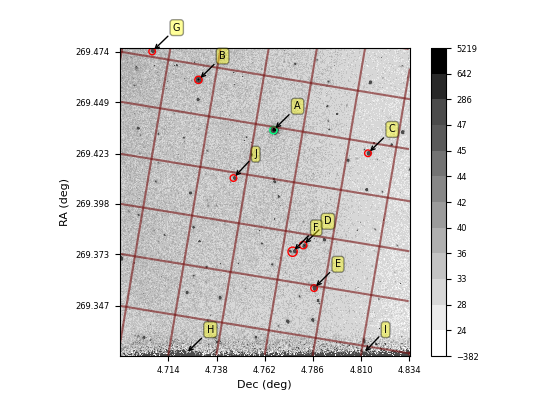
\includegraphics[scale=1]{images/initgexample.png}
\end{center}   
\caption{This is an observation of {\bstar} taken with the \texttt{g} filter on
17 September 2018 at 02:58:52 UTC after processing using the master bias and
flat files for September 2018. The brightest object, marked \textbf{A} and marked in
green is \bstar, whilst the next 9 brightest objects are marked in yellow and
\textbf{B}, \textbf{C}, etc. in decreasing order of brightness.}
\protect\label{fig:initgexample}
\end{figure}

\begin{figure}[!htbp]
\begin{center}
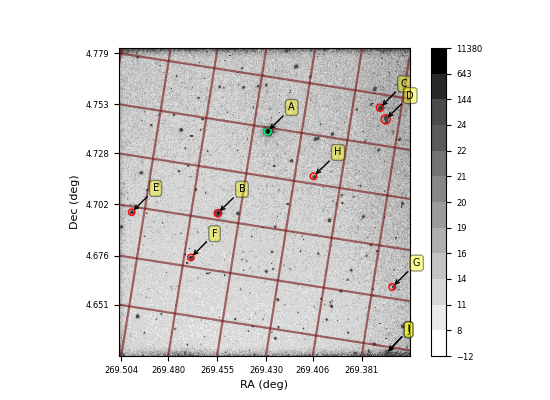
\includegraphics[scale=1]{images/initgexample20.png}
\end{center}   
\caption{This is an observation of {\bstar} taken with the \texttt{g} filter on
7 March 2020 at 09:07:23 UTC after processing using the master bias and
flat files for March 2020. The brightest object, marked \textbf{A} and marked in
green is \bstar, whilst the next 9 brightest objects are marked in yellow and
\textbf{B}, \textbf{C}, etc. in decreasing order of brightness.}
\protect\label{fig:initgexample20}
\end{figure}

In nearly every case there are 4 images taken, one with each of the 4 visible
light filters (in addition to the simultaneous REMIR observations) and in Fig.
\ref{fig:initgexample} is illustrated a set of observations of {\prox} taken on
the same date, 17 September 2018 as the observation of {\bstar} in Fig.
\ref{fig:initgexample}. For comparison, in Fig. \ref{fig:init4example20} is
shown a set of observations taken on 9 March 2020.

\begin{figure}[!htbp]
\begin{center}
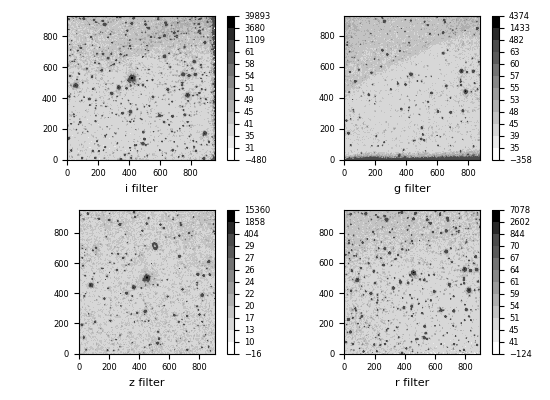
\includegraphics[scale=1]{images/init4example.png}
\end{center}   
\caption{This is all 4 observations of {\prox} taken with the visible light
filters on 17 September 2018 at 02:12:40 UTC after processing using
appropriate master bias and flat files for September 2018. They are arranged in
the order and orientation in which they are taken from the CCD. The
divisions on each image are pixel numbers.}
\protect\label{fig:init4example}
\end{figure}

\begin{figure}[!htbp]
\begin{center}
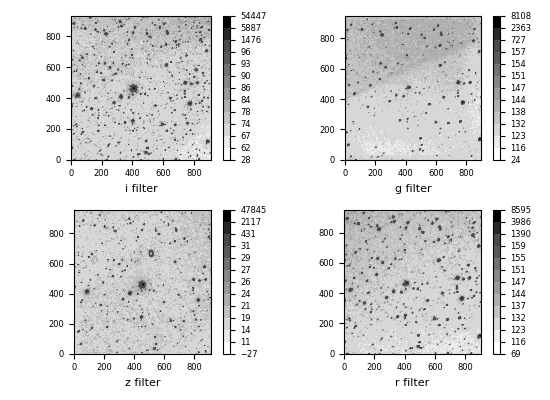
\includegraphics[scale=1]{images/init4example20.png}
\end{center}   
\caption{This is all 4 observations of {\prox} taken with the visible light
filters on 9 March 2020 at 08:56:14 UTC after processing using
appropriate master bias and flat files for March 2020. They are arranged in
the order and orientation in which they are taken from the CCD. The
divisions on each image are pixel numbers.}
\protect\label{fig:init4example20}
\end{figure}

\subsubsection{Some sample light curves}
\protect\label{section:samplelightcurves}

In Fig. \ref{fig:lcurvesing} is presented light curves of ADUs from {\prox}
from the observations on 16 and 17 September 2018 for the \texttt{g} and
\texttt{r} filters. In Fig. \ref{fig:lcurveref} is shown the same observations
where the ADUs are divided by the total ADUs of a subset of objects common to
all of the the other observations.

\begin{figure}[!htbp]
\begin{center}
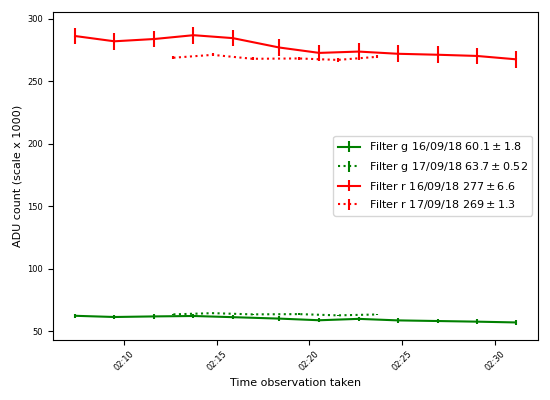
\includegraphics[scale=1]{images/demo_lcurve.png}
\end{center}   
\caption{This shows the total ADUs from the observations of {\prox} on 16 and
17 September 2018 for the \texttt{r} and \texttt{g} filters. The plot for each
day is overlaid to show the time taken.The results for those filters are in the appropriate colours with the later date dotted.}
\protect\label{fig:lcurvesing}
\end{figure}

\begin{figure}[!htbp]
\begin{center}
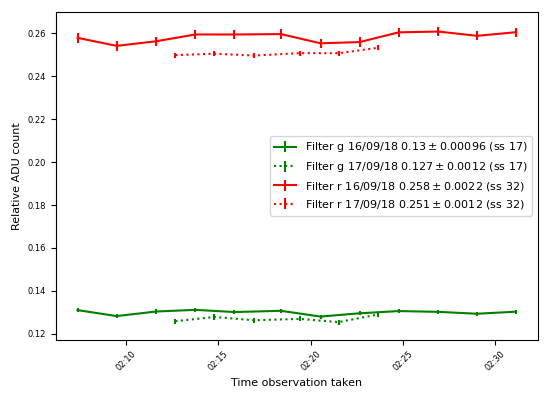
\includegraphics[scale=1]{images/demo_lcurve_refs.png}
\end{center}
\caption{This shows the total ADUs from the observations of {\prox} on 16 and
17 September 2018 for the \texttt{r} and \texttt{g} filters, (the same as in
Fig. \ref{fig:lcurvesing}) divided by the total of the ADUs for a subset of
other objects common to all the observations. The legend in each case shows the
subset size of the reference objects. }
\protect\label{fig:lcurveref}
\end{figure}

\clearpage

\subsection{Point spread functions}
\protect\label{section:pointspreadfunc}

In Fig. \ref{fig:im3d} is shown a 3D representation of the \texttt{g} filter
observation of {\prox} shown in Fig. \ref{fig:init4example}.

\textit{I plan to zoom in on some of the objects showing the cross-section in
various planes to illustrate that the objects are close to Gaussian in profile.
I then show how I can optimise the aperture for the objects to give an
acceptable accuracy across various frames. Also note that circular apertures
are sufficient, sufficiently few would benefit from using an elliptical
aperture to merit time being spent on these.}

\begin{figure}[!htbp]
\begin{center}
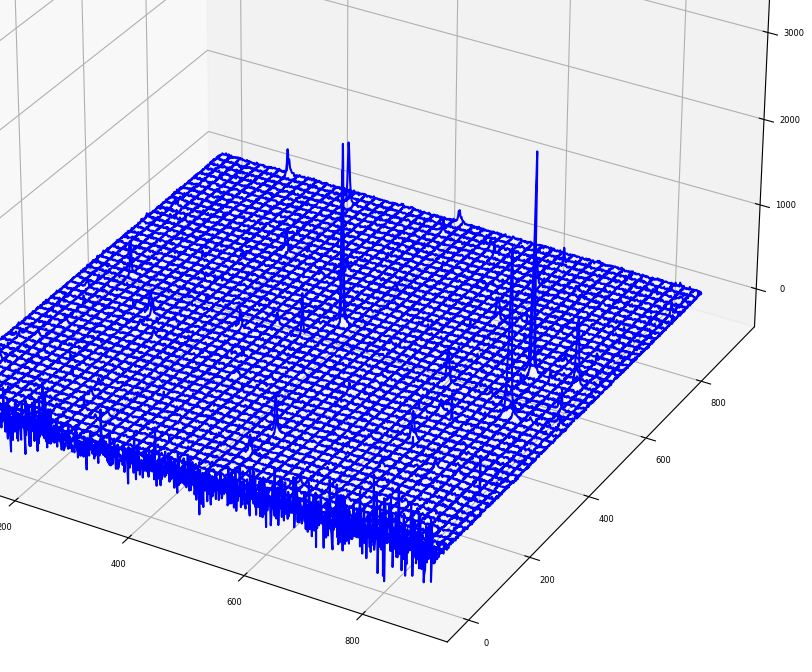
\includegraphics[scale=0.5]{images/im3d.png}
\end{center}
\caption{This is a 3-D representation of the \texttt{g} filter observation of
{\prox} already shown in Fig. \ref{fig:init4example} illustrating the peaks of
some of the objects.} \protect\label{fig:im3d}
\end{figure}

\clearpage

\subsection{Matters addressed in analysing data}
\protect\label{section:mattersaddressed}

The results of the initial processing of the data as discussed above highlighted
the matters which should be addressed to accurately process the images.

\subsubsection{Uncertainty measure}
\protect\label{section:issueuncertainty}

The light curves shown in Fig. \ref{fig:lcurvesing} and Fig. \ref{fig:lcurveref}
have error bars shown according to the standard deviation of the ADU count and
the ratio to the reference stars respectively. Given that the observations are
taken over an initial period of at most 20 minutes, it is unsurprising that
these do not vary much. Part of the variations which are shown may be due to
varying noise in the pixels on the CCD which are different for each exposure.

However the observations are all using the same master flat and bias files. It
is not clear what the uncertainty is on those files, so some analysis is
necessary.

\subsubsection{Flat files}
\protect\label{section:issueflatfiles}

It is of concern that there is a shading towards the bottom of the image; this
is the \texttt{g} filter, for which the bottom part of the image is taken from
the central part of the CCD (the \texttt{g} filter image is taken from the
upper right portion of the CCD, with the origin close to the centre of the CCD).
In Fig. \ref{fig:init4example} is the set of all visible light observations of
\prox, taken on the same date as in Fig. \ref{fig:initgexample} of 17 September 2018 at
02:12:40 UTC, with the images displayed in the sequence in which they are taken
from the CCD. For comparison, the same observations, without application of the
flat fields (but still with subtraction of the bias fields), are presented in
Fig. \ref{fig:init4exnoflat}. Also for comparison, in Fig.
\ref{fig:init4example20}, are observations of {\prox} parallel to those in Fig.
\ref{fig:init4example} from March 2020.

\begin{figure}[!htbp]
\begin{center}
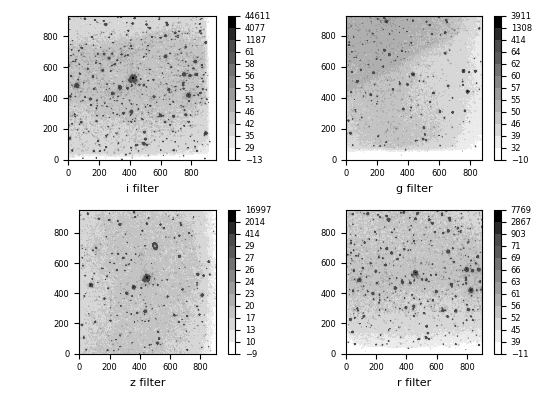
\includegraphics[scale=1]{images/init4exnoflat.png}
\end{center}   
\caption{This is all 4 observations of {\prox} taken with the visible light
filters on 17 September 2018 at 02:12:40 UTC, the same as in Fig.
\ref{fig:init4example}, after processing using appropriate master bias but
omitting the flat files for September 2018. The divisions on each image are pixel numbers.}
\protect\label{fig:init4exnoflat}
\end{figure}

It can be seen that the shading at the sides of the images is introduced by
applying the master flat fields.

\subsubsection{Negative pixels}
\protect\label{section:issuenegpixels}

Of additional concern is that a number of the pixel values are
negative after subtracting the bias value for each pixel. This in some cases is
larger than the pixel value at the same location in the observation file.
It would be expected that the bias level, with exposure of zero, should be
everywhere lower than any pixel observing sky, but this is not the case. For the images shown in Fig.
\ref{fig:init4example} the number of negative pixels are as shown in Table
\ref{table:initexnegpix}.

\begin{table}[!htbp]
\begin{center}
\begin{tabular}{lrrr} \hline
Filter & No of pixels & No negative & \% \\\hline
g & 818,296 & 763 & 0.09 \\
r & 858,600 & 388 & 0.05 \\
i & 898,560 & 2,143 & 0.24 \\
z & 866,136 & 1,401 & 0.16 \\
Total & 3,441,592 & 4,695 & 0.14 \\

\hline
\end{tabular}
\end{center}
\caption{Negative pixels in the images shown in Fig. \ref{fig:init4example} for
the various filters.}.
\protect\label{table:initexnegpix}
\end{table}

\subsubsection{Other caveats}
\protect\label{section:otherissues}

Of some concern is the ring shaped artefact above and slightly to the right of
the brightest objects in the images for the \texttt{z} filter, invariably for
the target, but to a greater or lesser degree for the other objects. Often the
artefact lands entirely on another object, compromising the usability of the
frame.

The \texttt{z} filter is poorest in terms of other objects in the frame for all
of the objects and there are few objects to be found in common subsets across
all the frame, this being because, despite being classified as ``visible
light'', it is in the near Infrared and the {\rdwarf} targets are much brighter
in this band then the other objects.

As a result, it proved advisable to avoid the \texttt{z} filter as it would not
be practical to try to compensate for the artefact given the likely poor return
if this were done. In any case the this is often worst or next to worst in terms
of the number of the negative pixels are to be found in the observations from
this filter, as shown in Table \ref{table:initexnegpix}.

\clearpage
